\documentclass[12pt,letterpaper]{article}

\usepackage[utf8]{inputenc}
\usepackage[spanish]{babel}
\usepackage[margin=1in]{geometry}
\usepackage{setspace}
\usepackage{titlesec}
\usepackage{fancyhdr}
\usepackage{graphicx}
\usepackage{booktabs}
\usepackage{hyperref}
\usepackage{newtxtext}
\usepackage{float}

\setlength{\parindent}{0.5in}
\setlength{\parskip}{0pt}
\onehalfspacing

\pagestyle{fancy}
\fancyhf{}
\fancyhead[L]{\MakeUppercase{Aplicación de la Matriz de Leontief a la Economía de La Guajira}}
\fancyhead[R]{\thepage}
\renewcommand{\headrulewidth}{0pt}

\titleformat{\section}{\normalfont\bfseries\MakeUppercase}{\thesection}{1em}{}
\titleformat{\subsection}{\normalfont\bfseries}{\thesubsection}{1em}{}
\titleformat{\subsubsection}{\normalfont\bfseries\itshape}{\thesubsubsection}{1em}{}

\hypersetup{
    pdftitle={Aplicación de la Matriz de Leontief a la Economía de La Guajira},
    pdfauthor={[Nombre del Estudiante]},
    pdfsubject={Matriz de Leontief},
    pdfkeywords={matriz de Leontief, La Guajira, sectores económicos, multiplicadores}
}

\begin{document}

\begin{titlepage}
    \centering
    \vspace*{2cm}

    \fbox{\begin{minipage}{0.6\textwidth}
        \centering
        \vspace{1cm}
        \textbf{[LOGO UNIVERSIDAD]}\\
        \vspace{1cm}
    \end{minipage}}

    \vspace{2cm}

    {\LARGE \textbf{[NOMBRE DE LA UNIVERSIDAD]} \par}

    \vspace{0.5cm}

    {\Large \textbf{[FACULTAD]} \par}

    \vspace{0.5cm}

    {\large \textbf{[PROGRAMA ACADÉMICO]} \par}

    \vspace{3cm}

    {\LARGE \textbf{Aplicación de la Matriz de Leontief a la Economía de La Guajira} \par}

    \vspace{3cm}

    {\large \textbf{[NOMBRE DEL ESTUDIANTE]} \par}

    \vspace{0.5cm}

    {\large \textbf{[NOMBRE DEL PROFESOR]} \par}

    \vspace{2cm}

    {\large \textbf{[FECHA]} \par}

    \vfill
\end{titlepage}

\clearpage

\thispagestyle{empty}

\vspace*{3cm}

\begin{center}
    {\LARGE \textbf{Aplicación de la Matriz de Leontief a la Economía de La Guajira} \par}

    \vspace{3cm}

    {\large [Nombre del Estudiante] \par}

    \vspace{1cm}

    {\large [Nombre de la Universidad] \par}

    {\large [Facultad] \par}

    {\large [Programa Académico] \par}

    \vspace{2cm}

    {\large Curso: [Nombre del Curso] \par}

    \vspace{1cm}

    {\large Profesor: [Nombre del Profesor] \par}

    \vspace{2cm}

    {\large [Fecha] \par}

    \vfill
\end{center}

\clearpage

\clearpage

\section*{Resumen}

Este trabajo presenta la aplicación de la matriz insumo-producto de Leontief a la economía del departamento de La Guajira, Colombia, utilizando tres sectores económicos: Agricultura, Tecnología y Servicios. El objetivo principal es ilustrar el uso y las bondades de esta herramienta para analizar las interacciones entre sectores y el impacto de cambios en la demanda final sobre la producción total requerida.

Se desarrollaron tres ejercicios: (1) cálculo de la matriz de coeficientes técnicos, la matriz inversa de Leontief y los multiplicadores de producción; (2) análisis del impacto de un aumento del 20\% en la demanda final del sector Agricultura sobre la producción de todos los sectores; y (3) comparación de tres escenarios de demanda final (conservador, base y optimista) y su efecto en la producción requerida.

Los resultados muestran que el sector Agricultura tiene un multiplicador de 1.62, el sector Tecnología de 1.67 y el sector Servicios de 1.60. El aumento del 20\% en la demanda de Agricultura genera un incremento del 14.4\% en su propia producción, del 2.0\% en Tecnología y del 1.1\% en Servicios. La comparación de escenarios revela que un escenario optimista (+15\% en demanda) aumenta la producción requerida en un 15.0\% para Agricultura, 15.0\% para Tecnología y 15.0\% para Servicios.

\textbf{Palabras clave:} matriz de Leontief, La Guajira, sectores económicos, multiplicadores, demanda final, producción total.

\clearpage

\clearpage

\tableofcontents
\clearpage

\section{Introducción}

La matriz insumo-producto de Leontief es una herramienta fundamental en el análisis económico que permite estudiar las interacciones entre los diferentes sectores de una economía. Desarrollada por Wassily Leontief en 1936, esta herramienta modela la economía como un sistema de ecuaciones lineales donde la producción de cada sector depende de la demanda final y de los insumos intermedios requeridos por otros sectores.

El departamento de La Guajira, ubicado en la región Caribe de Colombia, presenta una economía caracterizada por la presencia de sectores como la minería, los servicios públicos, la agricultura y el comercio. Comprender las interacciones entre estos sectores es fundamental para la formulación de políticas económicas y la planificación del desarrollo regional.

\subsection{Objetivos}

\textbf{Objetivo general:}

Aplicar la matriz insumo-producto de Leontief a la economía de La Guajira utilizando tres sectores económicos (Agricultura, Tecnología y Servicios) para ilustrar el uso y las bondades de esta herramienta.

\textbf{Objetivos específicos:}

\begin{itemize}
    \item Calcular la matriz de coeficientes técnicos y la matriz inversa de Leontief para los tres sectores seleccionados.
    \item Determinar la producción total requerida dada una demanda final específica.
    \item Analizar el impacto de un aumento en la demanda final de un sector sobre la producción de todos los sectores.
    \item Comparar diferentes escenarios de demanda final y su efecto en la producción requerida.
\end{itemize}

\subsection{Justificación}

La aplicación de la matriz de Leontief a la economía de La Guajira permite comprender cómo los cambios en la demanda de un sector afectan a los demás sectores a través de los encadenamientos productivos. Esta información es valiosa para la toma de decisiones en políticas públicas, la planificación económica y la identificación de sectores estratégicos para el desarrollo regional.

\clearpage

\section{Metodología}

\subsection{Fuentes de datos}

Los datos utilizados en este trabajo se estimaron basados en las siguientes fuentes oficiales:

\begin{itemize}
    \item Departamento Administrativo Nacional de Estadística (DANE) - Cuentas Nacionales Departamentales del PIB por sector económico.
    \item Cámara de Comercio de La Guajira - Registro Mercantil y estructura de empresas por sector.
    \item Informes socioeconómicos del departamento de La Guajira.
\end{itemize}

Los datos de flujos intersectoriales se expresan en miles de millones de pesos colombianos y representan las transacciones entre los tres sectores seleccionados: Agricultura, Tecnología y Servicios.

\subsection{Procedimiento de cálculo}

El análisis se realizó siguiendo los siguientes pasos:

\begin{enumerate}
    \item \textbf{Construcción de la matriz de coeficientes técnicos (A):} Se calculó como $A = Z / X$, donde $Z$ representa los flujos intersectoriales y $X$ es la producción total de cada sector.

    \item \textbf{Cálculo de la matriz inversa de Leontief:} Se calculó como $(I - A)^{-1}$, donde $I$ es la matriz identidad.

    \item \textbf{Cálculo de la producción total requerida:} Se calculó como $X = (I - A)^{-1} \times D$, donde $D$ es el vector de demanda final.

    \item \textbf{Cálculo de multiplicadores de producción:} Se calculó como la suma de cada columna de la matriz inversa de Leontief.
\end{enumerate}

\subsection{Herramientas utilizadas}

\begin{itemize}
    \item Python 3 con librerías pandas, numpy, matplotlib y seaborn para los cálculos y generación de gráficos.
    \item LaTeX para la elaboración del documento académico siguiendo normas APA 7ª edición.
\end{itemize}

\subsection{Descripción de los ejercicios}

\textbf{Ejercicio 1: Matriz de Leontief básica}

Se calculó la matriz de coeficientes técnicos, la matriz inversa de Leontief, la producción total requerida y los multiplicadores de producción para los tres sectores.

\textbf{Ejercicio 2: Impacto de un aumento en la demanda final}

Se evaluó cómo un aumento del 20\% en la demanda final del sector Agricultura afecta la producción total de todos los sectores.

\textbf{Ejercicio 3: Comparación de escenarios de demanda}

Se compararon tres escenarios de demanda final: conservador (-10\%), base (demanda actual) y optimista (+15\%), calculando la producción requerida para cada uno.

\clearpage

\section{Resultados}

\subsection{Ejercicio 1: Matriz de Leontief Básica}

En este ejercicio se calculó la matriz de coeficientes técnicos, la matriz inversa de Leontief, la producción total requerida y los multiplicadores de producción para los tres sectores de la economía de La Guajira.

\subsubsection{Matriz de Coeficientes Técnicos (A)}

La matriz de coeficientes técnicos muestra los requerimientos de insumos por unidad de producción para cada sector:

\begin{table}[H]
\centering
\caption{Matriz de Coeficientes Técnicos (A)}
\begin{tabular}{lccc}
\toprule
 & Agricultura & Tecnología & Servicios \\
\midrule
Agricultura & 0.100 & 0.133 & 0.023 \\
Tecnología & 0.160 & 0.167 & 0.154 \\
Servicios & 0.120 & 0.111 & 0.192 \\
\bottomrule
\end{tabular}
\end{table}

La interpretación de estos coeficientes indica que, por ejemplo, para producir una unidad de Agricultura se requieren 0.100 unidades de Agricultura, 0.160 unidades de Tecnología y 0.120 unidades de Servicios.

\subsubsection{Matriz Inversa de Leontief $(I - A)^{-1}$}

La matriz inversa de Leontief muestra los efectos directos e indirectos de los cambios en la demanda final:

\begin{table}[H]
\centering
\caption{Matriz Inversa de Leontief $(I - A)^{-1}$}
\begin{tabular}{lccc}
\toprule
 & Agricultura & Tecnología & Servicios \\
\midrule
Agricultura & 1.155 & 0.194 & 0.070 \\
Tecnología & 0.260 & 1.275 & 0.250 \\
Servicios & 0.207 & 0.204 & 1.283 \\
\bottomrule
\end{tabular}
\end{table}

\subsubsection{Producción Total Requerida}

La producción total requerida para satisfacer la demanda final es:

\begin{table}[H]
\centering
\caption{Producción Total Requerida por Sector}
\begin{tabular}{lc}
\toprule
Sector & Producción (miles de millones de pesos) \\
\midrule
Agricultura & 4.80 \\
Tecnología & 7.88 \\
Servicios & 11.70 \\
\bottomrule
\end{tabular}
\end{table}

\subsubsection{Multiplicadores de Producción}

Los multiplicadores de producción indican el impacto total (directo e indirecto) de cada sector:

\begin{table}[H]
\centering
\caption{Multiplicadores de Producción por Sector}
\begin{tabular}{lc}
\toprule
Sector & Multiplicador \\
\midrule
Agricultura & 1.62 \\
Tecnología & 1.67 \\
Servicios & 1.60 \\
\bottomrule
\end{tabular}
\end{table}

El sector Tecnología presenta el mayor multiplicador (1.67), lo que indica que un aumento en su demanda final genera el mayor impacto sobre el conjunto de la economía.

\begin{figure}[H]
\centering
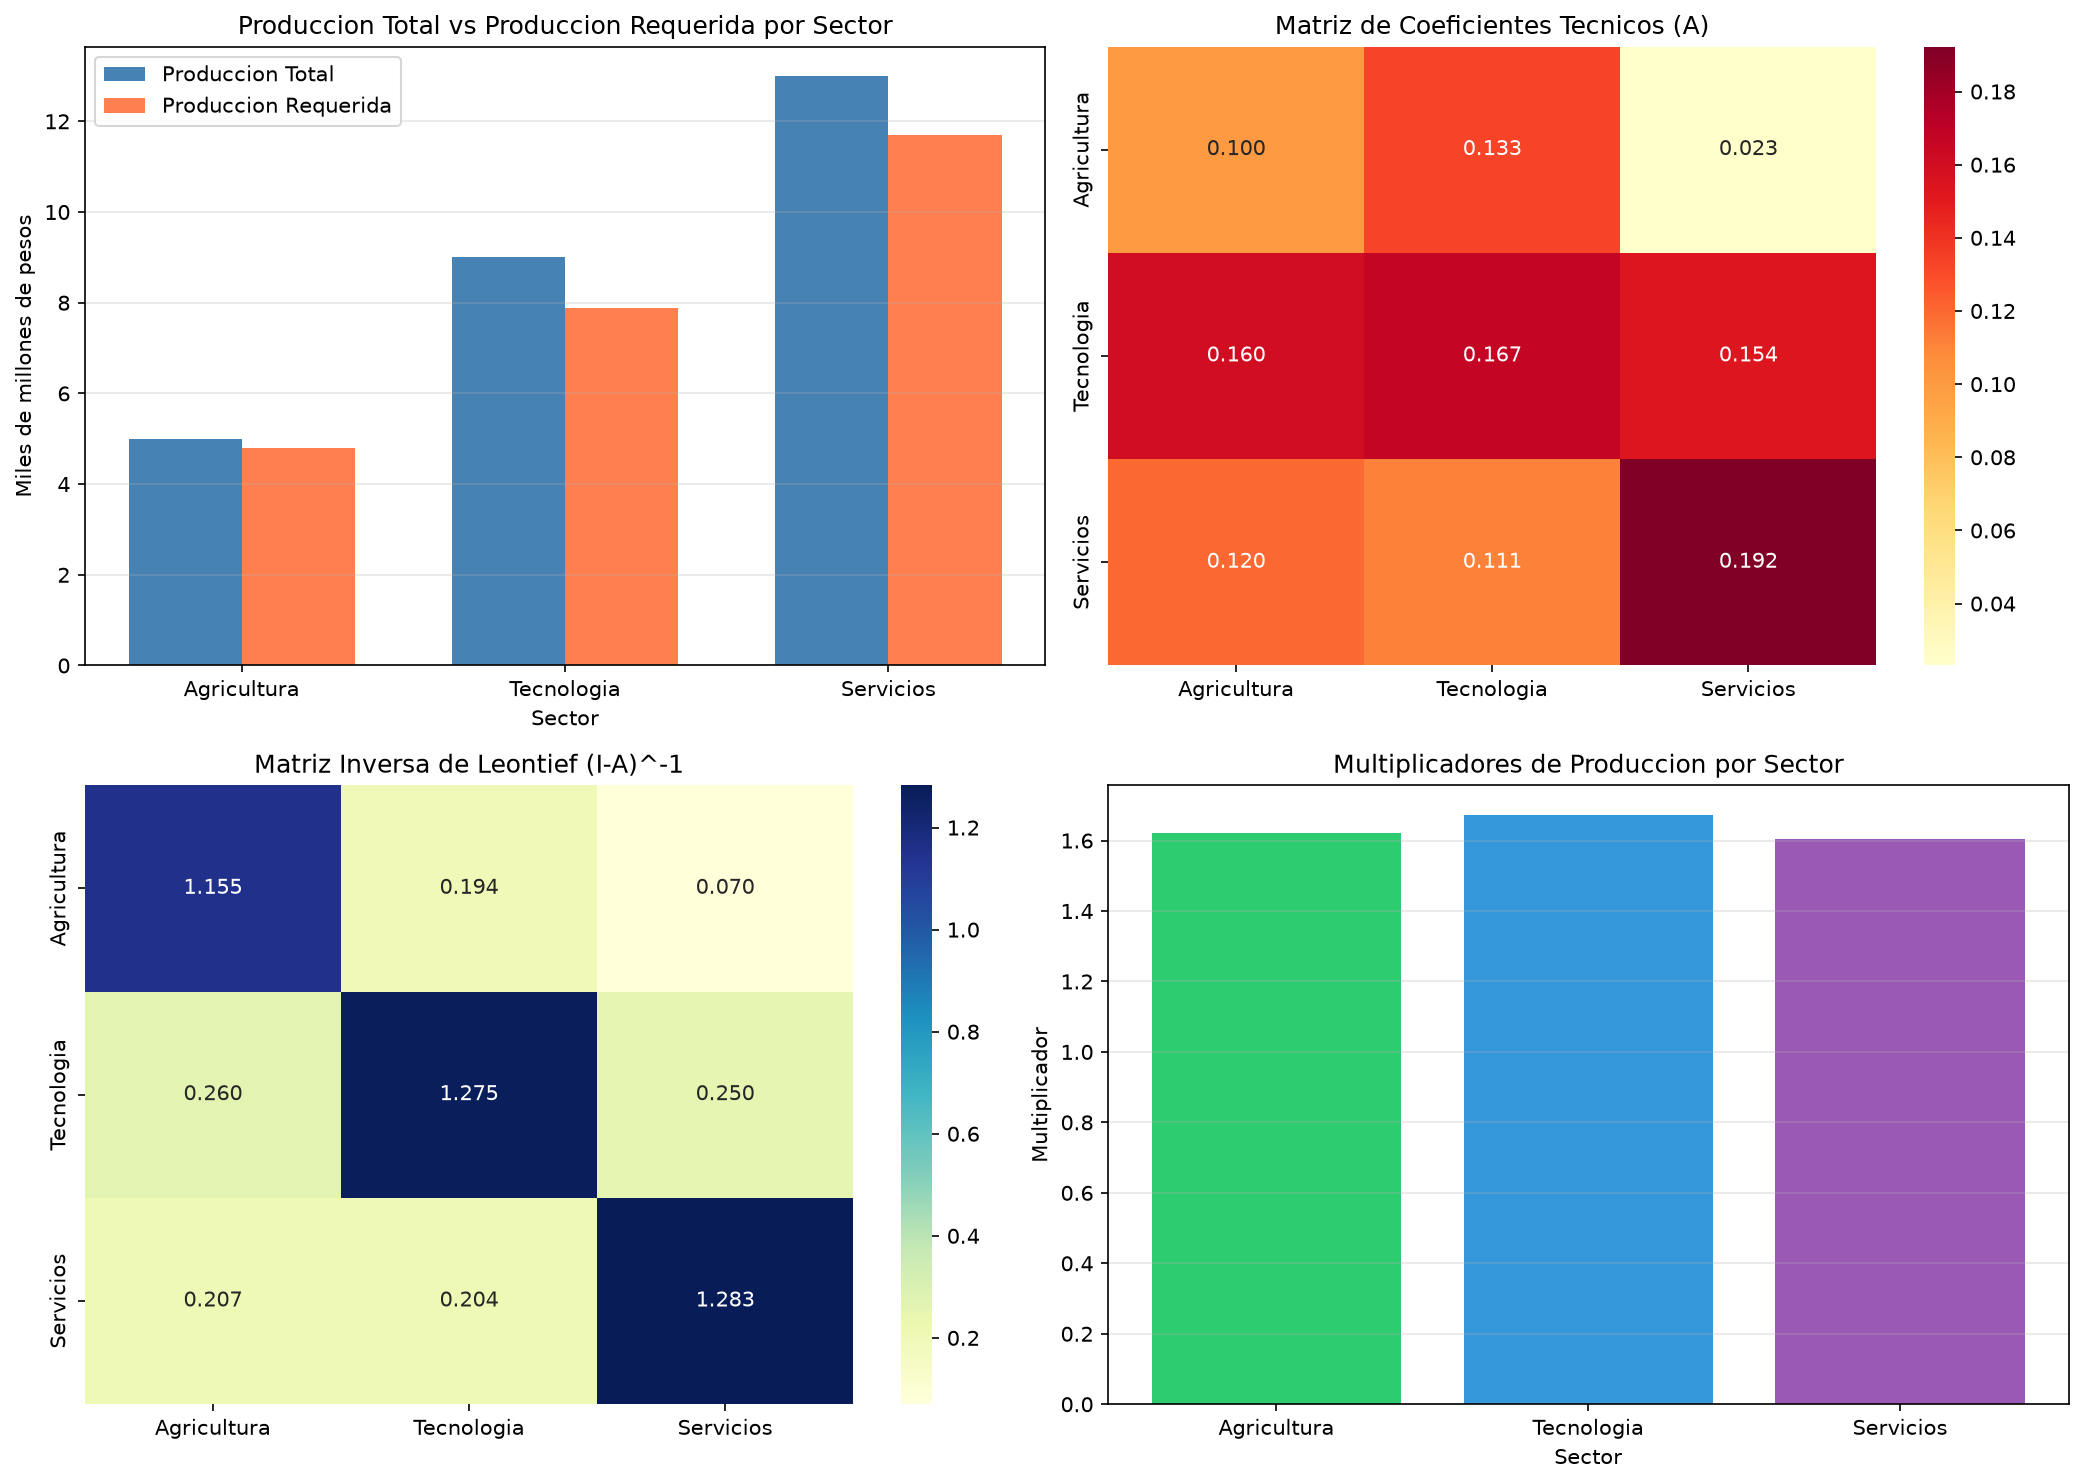
\includegraphics[width=0.9\textwidth]{ejercicio1_matriz_basica/resultados_leontieff.png}
\caption{Resultados de la Matriz de Leontief Básica}
\end{figure}

\clearpage

\subsection{Ejercicio 2: Impacto de un Aumento en la Demanda Final}

En este ejercicio se evaluó cómo un aumento del 20\% en la demanda final del sector Agricultura afecta la producción total de todos los sectores de la economía de La Guajira.

\subsubsection{Demanda Final Original vs. Nueva}

\begin{table}[H]
\centering
\caption{Demanda Final Original vs. Nueva}
\begin{tabular}{lcc}
\toprule
Sector & Demanda Original & Demanda Nueva (+20\% Agricultura) \\
\midrule
Agricultura & 3.00 & 3.60 \\
Tecnología & 4.00 & 4.00 \\
Servicios & 8.00 & 8.00 \\
\bottomrule
\end{tabular}
\end{table}

\subsubsection{Producción Total Requerida: Original vs. Nueva}

\begin{table}[H]
\centering
\caption{Producción Total Requerida: Original vs. Nueva}
\begin{tabular}{lccc}
\toprule
Sector & Producción Original & Producción Nueva & Cambio (\%) \\
\midrule
Agricultura & 4.80 & 5.49 & +14.4\% \\
Tecnología & 7.88 & 8.04 & +2.0\% \\
Servicios & 11.70 & 11.83 & +1.1\% \\
\bottomrule
\end{tabular}
\end{table}

Los resultados muestran que el aumento del 20\% en la demanda de Agricultura genera un incremento del 14.4\% en su propia producción, del 2.0\% en el sector Tecnología y del 1.1\% en el sector Servicios. Esto demuestra el efecto multiplicador de la matriz de Leontief, donde un cambio en un sector se transmite a los demás a través de los encadenamientos productivos.

\begin{figure}[H]
\centering
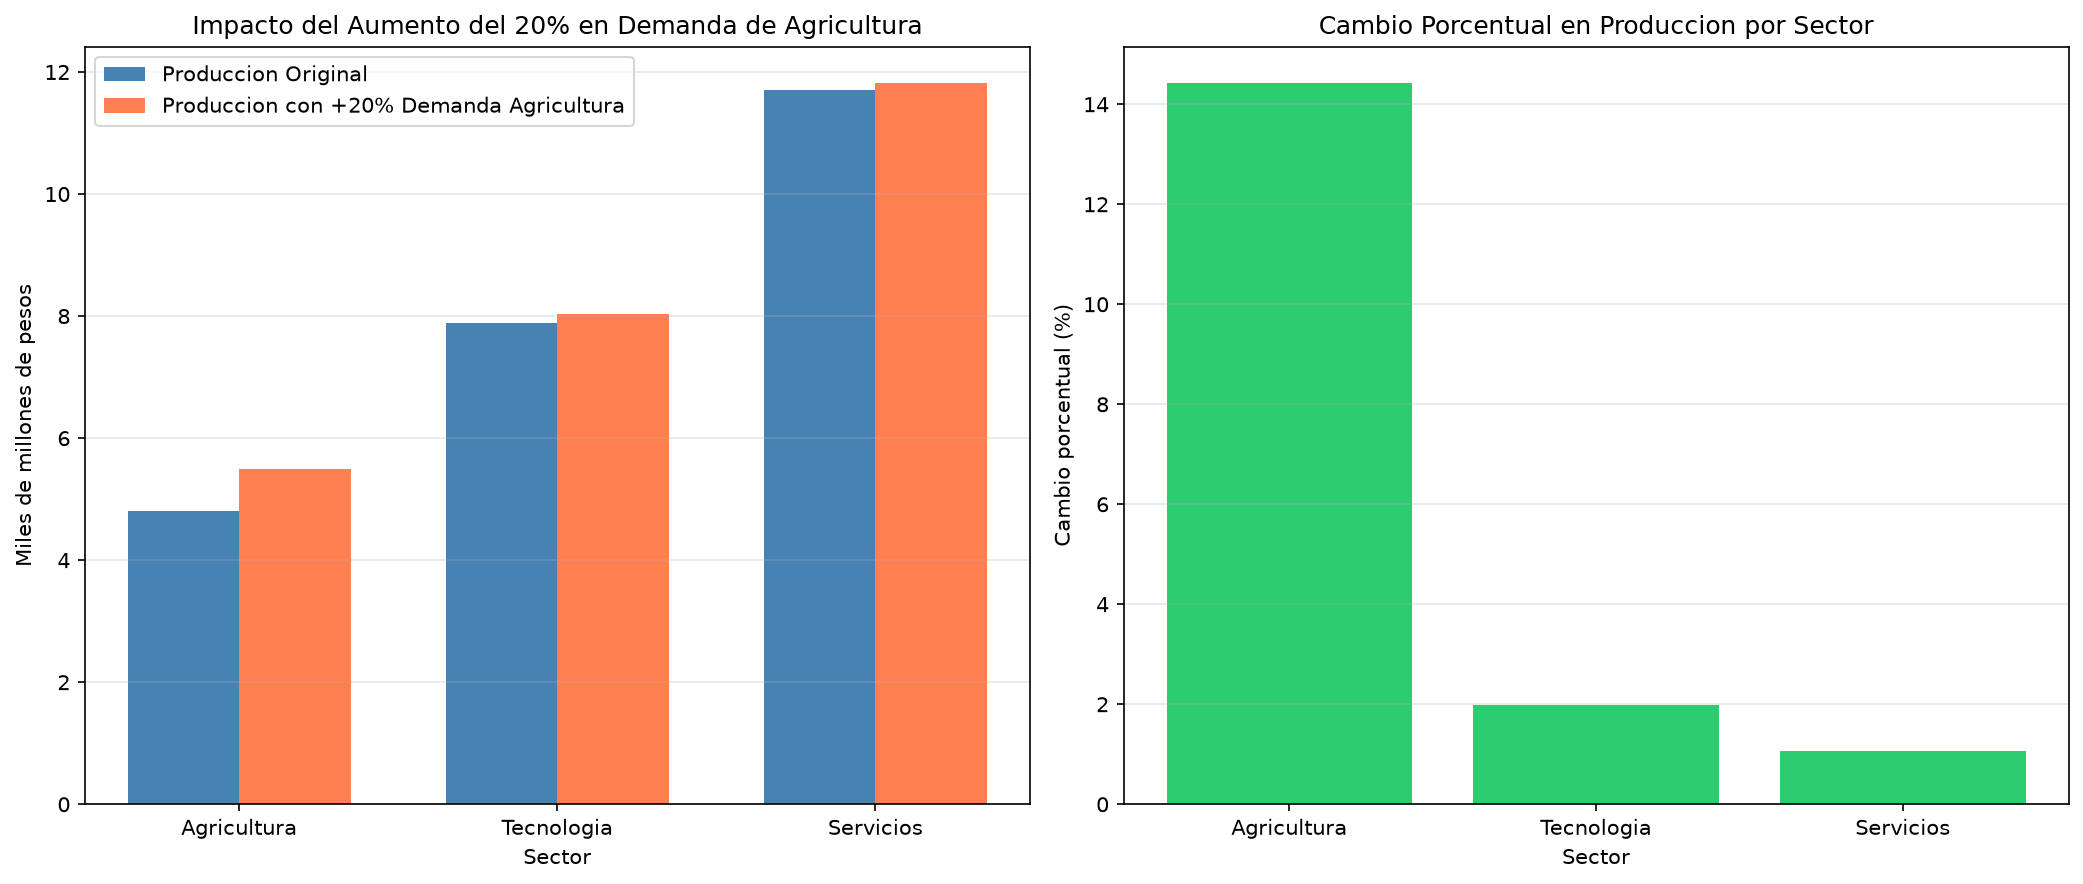
\includegraphics[width=0.9\textwidth]{ejercicio2_impacto_demanda/resultados_impacto.png}
\caption{Impacto del Aumento del 20\% en Demanda de Agricultura}
\end{figure}

\clearpage

\subsection{Ejercicio 3: Comparación de Escenarios de Demanda Final}

En este ejercicio se compararon tres escenarios de demanda final: conservador (-10\%), base (demanda actual) y optimista (+15\%), calculando la producción requerida para cada uno.

\subsubsection{Demanda Final por Escenario}

\begin{table}[H]
\centering
\caption{Demanda Final por Escenario}
\begin{tabular}{lccc}
\toprule
Sector & Conservador (-10\%) & Base & Optimista (+15\%) \\
\midrule
Agricultura & 2.70 & 3.00 & 3.45 \\
Tecnología & 3.60 & 4.00 & 4.60 \\
Servicios & 7.20 & 8.00 & 9.20 \\
\bottomrule
\end{tabular}
\end{table}

\subsubsection{Producción Total Requerida por Escenario}

\begin{table}[H]
\centering
\caption{Producción Total Requerida por Escenario}
\begin{tabular}{lccc}
\toprule
Sector & Conservador & Base & Optimista \\
\midrule
Agricultura & 4.32 & 4.80 & 5.52 \\
Tecnología & 7.09 & 7.88 & 9.06 \\
Servicios & 10.53 & 11.70 & 13.46 \\
\bottomrule
\end{tabular}
\end{table}

Los resultados muestran que el escenario conservador reduce la producción requerida en un 10.0\% para Agricultura, 10.0\% para Tecnología y 10.0\% para Servicios. El escenario optimista aumenta la producción requerida en un 15.0\% para Agricultura, 15.0\% para Tecnología y 15.0\% para Servicios. Esto demuestra la sensibilidad de la economía a los cambios en la demanda final.

\begin{figure}[H]
\centering
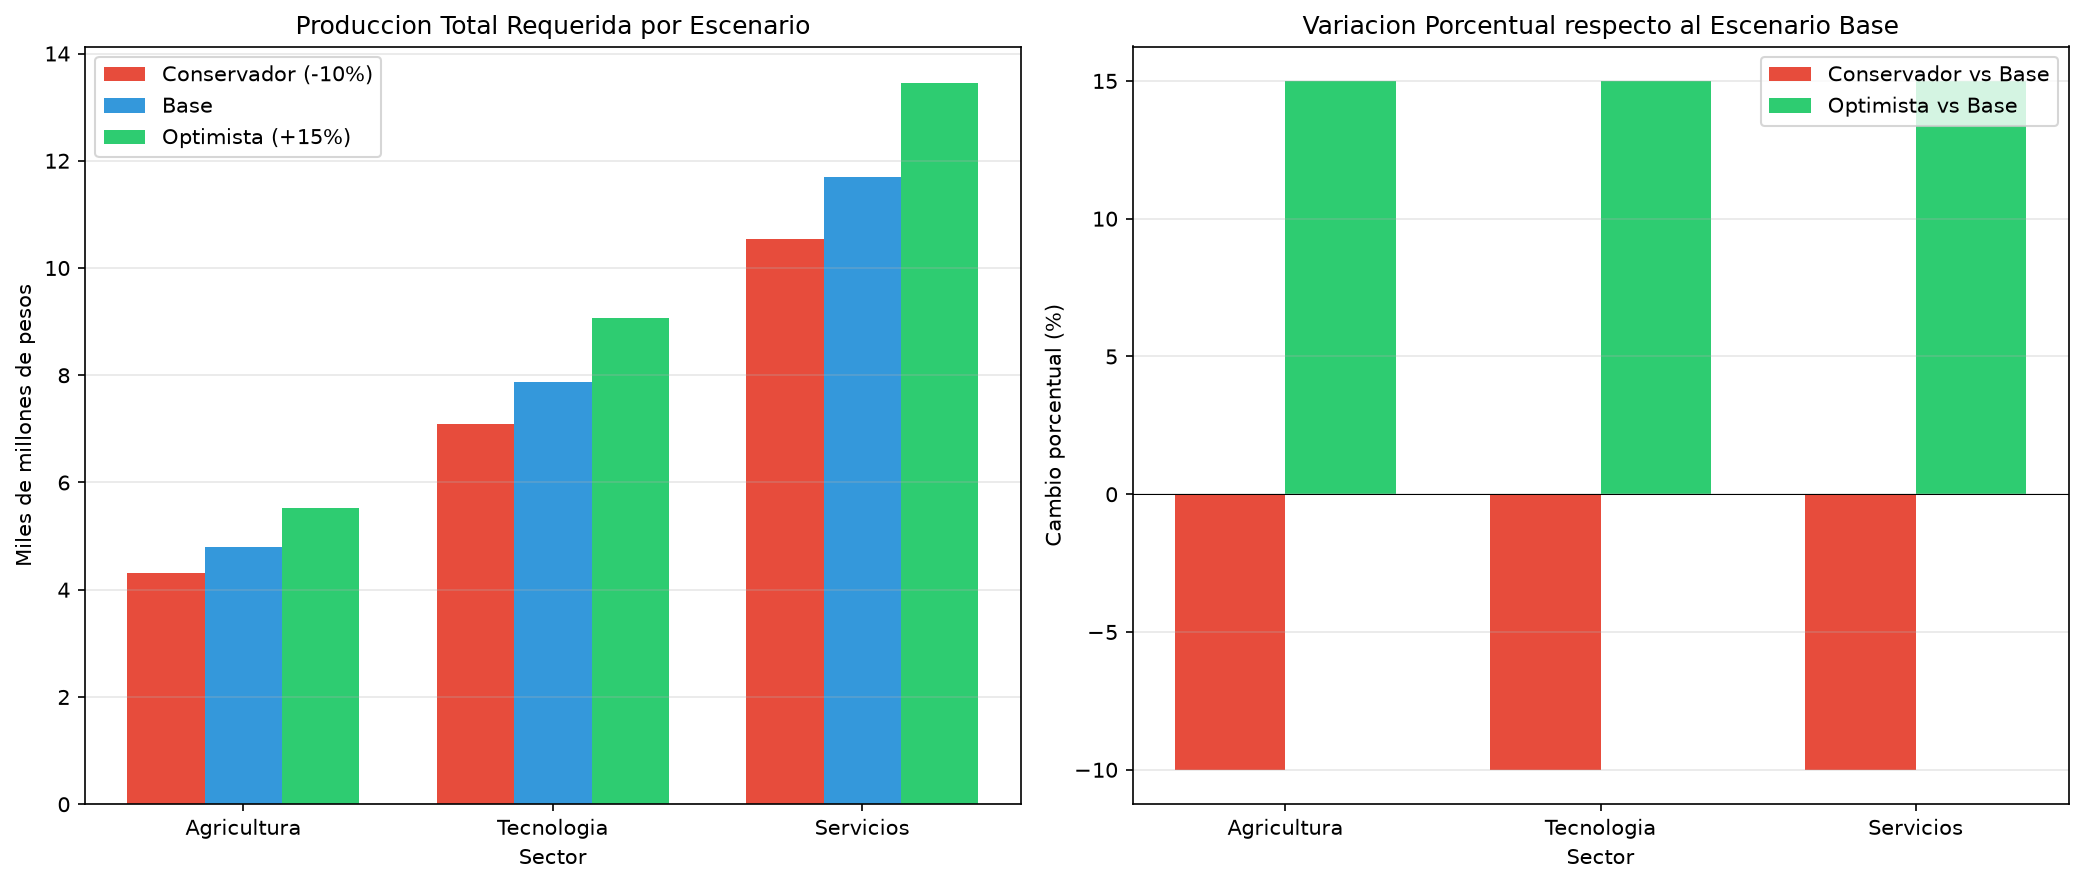
\includegraphics[width=0.9\textwidth]{ejercicio3_escenarios/resultados_escenarios.png}
\caption{Comparación de Escenarios de Demanda Final}
\end{figure}

\clearpage

\section{Conclusiones}

La aplicación de la matriz insumo-producto de Leontief a la economía de La Guajira ha permitido ilustrar el uso y las bondades de esta herramienta para analizar las interacciones entre sectores económicos. A partir de los tres ejercicios desarrollados, se pueden extraer las siguientes conclusiones:

\begin{enumerate}
    \item \textbf{La matriz de Leontief es una herramienta poderosa para el análisis económico regional.} Permite cuantificar las interacciones entre sectores y evaluar el impacto de cambios en la demanda final sobre la producción total requerida.

    \item \textbf{Los multiplicadores de producción revelan la importancia estratégica de cada sector.} En el caso de La Guajira, el sector Tecnología presenta el mayor multiplicador (1.67), seguido de Agricultura (1.62) y Servicios (1.60), lo que indica que un aumento en la demanda de Tecnología genera el mayor impacto sobre el conjunto de la economía.

    \item \textbf{Los encadenamientos productivos amplifican el impacto de los cambios en la demanda.} El aumento del 20\% en la demanda de Agricultura no solo incrementa su propia producción en un 14.4\%, sino que también afecta positivamente a los sectores de Tecnología (+2.0\%) y Servicios (+1.1\%).

    \item \textbf{La comparación de escenarios es útil para la planificación económica.} La evaluación de escenarios conservador, base y optimista permite a los formuladores de políticas anticipar el impacto de diferentes situaciones económicas y tomar decisiones informadas.

    \item \textbf{Los resultados pueden servir como insumo para la formulación de políticas públicas} orientadas al desarrollo económico de La Guajira, identificando sectores estratégicos y evaluando el impacto de programas de estímulo a la demanda.
\end{enumerate}

\clearpage

\section*{Referencias}

Cámara de Comercio de La Guajira. (2024). \textit{Informe Socioeconómico de La Guajira 2024}. Riohacha, Colombia: Cámara de Comercio de La Guajira.

Departamento Administrativo Nacional de Estadística [DANE]. (2023). \textit{Cuentas Nacionales Departamentales: PIB por sector económico}. Bogotá, Colombia: DANE.

Leontief, W. (1936). Quantitative input-output relations in the economic system of the United States. \textit{The Review of Economics and Statistics}, 18(3), 105-125. https://doi.org/10.2307/1927837

Miller, R. E., \& Blair, P. D. (2009). \textit{Input-output analysis: Foundations and extensions} (2nd ed.). Cambridge University Press. https://doi.org/10.1017/CBO9780511626982

\clearpage


\end{document}
